\documentclass{ProblemSetCUNY}
\usepackage{bussproofs} \EnableBpAbbreviations
\usepackage{mathrsfs}
\usepackage{stix}
\usepackage{pgffor}
\usepackage{listings}

\usepackage{amssymb}
\usepackage{booktabs}
\usepackage{array}
\usepackage{tikz}
\usetikzlibrary{automata, arrows.meta, positioning}

\usepackage{tabstackengine}
\TABstackMath
\TABbinary

\AssignmentNumber{3}%
\CourseName{Automation Engineering}
\CourseNumber{39531}
\InstructorName{Alex Washburn}
\DueDateYear{2026}
\DueDateMonth{02}
\DueDateDay{27}


%\newenvironment{\ContactListing}[args]{begdef}{enddef}

\newcommand{\Bool}{\ensuremath{\mathtt{Bool}}\xspace}
%\newcommand{\Nats}{\ensuremath{\mathbb{N}}\xspace}
%\newcommand{\Ints}{\ensuremath{\mathbb{Z}}\xspace}
%\newcommand{\Rats}{\ensuremath{\mathbb{Q}}\xspace}
%\newcommand{\Reals}{\ensuremath{\mathbb{R}}\xspace}
%\newcommand{\ProofLabelOne}[1]{\RightLabel{\ensuremath{\Parens{\mathrm{\textsc{#1}}}}\xspace}}
\newcommand{\ProofLabelTwo}[2]{\RightLabel{\ensuremath{\Parens{\mathrm{\textsc{#1}}}\Parens{\mathrm{#2}}}\xspace}}

\newcommand{\LogicCase}[1]{\item \textbf{Case}~#1:\newline}

\newcommand{\DerivationFormat}[2]{\hfill\qquad#2\textsc{#1}}
\newcommand{\Derivation}[2]{\DerivationFormat{#1}{#2~\ensuremath{\ruledelayed}~}}

\newcommand{\AxiomCL}[1]{\DerivationFormat{Axiom~#1}{}}
\newcommand{\Factivity}{\DerivationFormat{Factivity}{}}
\newcommand{\Given}{\DerivationFormat{Hypothesis}{}}
\newcommand{\Contrapositive}{\DerivationFormat{Contrapositive}{}}
\newcommand{\DoubleNegation}{\DerivationFormat{Double Negation}{}}
\newcommand{\DeMorgans}{\DerivationFormat{DeMorgans}{}}
\newcommand{\Necitation}[1]{\Derivation{Necitation}{#1}}
\newcommand{\Distribution}[1]{\Derivation{Distribution}{#1}}
\newcommand{\Reflexivity}[1]{\Derivation{Reflexivity}{#1}}
\newcommand{\ConDef}[1]{\Derivation{Connective Definition}{#1}}
\newcommand{\Contradiction}[1]{\ensuremath{\neg \phi \land \phi}\Derivation{Contradiction}{\ensuremath{\phi = #1}}}
\newcommand{\DedThm}[1]{\Derivation{Deduction Theorem}{#1}}
\newcommand{\ModPon}[2]{\Derivation{Modus Ponens}{#1, #2}}
\newcommand{\Syllogism}[2]{\Derivation{Syllogism}{#1, #2}}
\newcommand{\Theorem}[2]{\DerivationFormat{Theorem~--~Lecture~#1,~Page~#2}{}}

\newcommand{\R}[2]{\ensuremath{\World{#1}\mathrel{R}\World{#2}}\xspace}
\newcommand{\Tr}[2]{\ensuremath{\tau\Parens{#1,\,#2}\xspace}}
\newcommand{\T}[1]{\ensuremath{\tau\Parens{#1}\xspace}}
\newcommand{\Prob}[1]{\ensuremath{P\Parens{#1}}\xspace}
\newcommand{\ProbGiven}[2]{\ensuremath{P\Parens{#1~\,|\,~#2}}\xspace}
\newcommand{\RandVar}[1]{\ensuremath{\mathbf{#1}}\xspace}
\newcommand{\DistMap}[2]{~#1&\mapsto~~#2\\}
\newcommand{\DistCondition}[2]{~#1&\text{\normalfont iff}~~#2\\}


\newcommand{\One}{\ensuremath{\textbf{1}}\xspace}

\newcommand{\Cons}{%
\mathrel{:\!:}%
}

\newcommand{\ProblemItem}[1]{%
\hspace{\parindent}\textbullet\;\;#1%
}

\begin{document}
\CoverPage%


%
% Mapping
% Configuration updates
% Folding
%


\Problem{%
Ray Sonant wants to better understand the operation of a security door at his manufacturing facility so that they can be sure that the facility is secure.%
You are helping Ray model the security door's functionality using a Finite State Automata (FSA).%
The security door system includes:%
\ProblemItem{An electronic lock}\\
\ProblemItem{An intrusion alarm}\\
\ProblemItem{A keypad for credential entry}\\
\ProblemItem{A manual door push mechanism}\\[5mm]%
The controller receives the following finite set of input symbols:
$$\Sigma\;=\;\SetNote{\texttt{push},\, \texttt{invalid},\, \texttt{valid},\, \texttt{disable},\, \texttt{enable} }$$
Where:
\ProblemItem{\texttt{valid} -- a valid credential is entered}\\
\ProblemItem{\texttt{invalid} -- an invalid credential attempt}\\
\ProblemItem{\texttt{push} -- the door is physically pushed (attempt to open)}\\
\ProblemItem{\texttt{enable} -- the door is manually re-locked from an unlocked state}\\
\ProblemItem{\texttt{disable} -- alarm is manually disabled when it is sounding}\\[5mm]%
The manufacture's manual Ray Sonant gives you states the folowing \textbf{System Requirements}:\\
\ProblemItem{The system begins in the locked state.}\\
\ProblemItem{A valid input unlocks the door.}\\
\ProblemItem{A push opens the door \textit{only if it is unlocked}.}\\
\ProblemItem{While locked, three consecutive `invalid` attempts trigger the alarm.}\\
\ProblemItem{A valid attempt resets the invalid counter.}\\
\ProblemItem{When the alarm is sounding, it must be disabled before receiving any other input.}\\
\ProblemItem{From the Open state, enabling the security system returns the door to locked.}\\[5mm]%
\textit{Help Ray Sonant become confident in the door's security system by answering the questions on the next page.}
}%
\pagebreak
\SubProblem{What is the set of states $Q$ for Ray Sonant's security door?}
\vfill
\SubProblem{What is the starting state?}
\vfill
\SubProblem{What is/are the accepting state(s)?}
\vfill
\SubProblem{Draw a diagram of the FSA for Ray Sonant's security door.}
\vfill
\vfill
\vfill
\vfill
\vfill
\vfill


\Problem{%
Baron Finn Isham of the Principality of Sealand has commissioned Perry Scope to designed a missle launch system for the nation's self defense. %
Perry Scope has designed this kind of system before, and has a Finite State Automata (FSA) diagram on the next page. %
Unfortunately, Baron Finn Isham is weird and does not like pictures, only tables of instructions. %
Furthermore, Baron Finn Isham just wants proof that a missile can be launched in some sequence.\\[5mm]%
\textit{Help Perry Scope satisfy Baron Finn Isham by converting the FSA diagram to an FSA state transition table that lists \emph{\textbf{any}} sequence which goes from the the stating state to an accepting state (missile launched).}\\[5mm]%
\textit{Note:} Use tuple notation shorthand for the states in $\Tuple{x,\,y,\,z} \in Q$:\\%
\ProblemItem{$x \in \SetNote{O,\,C}$ for lid is \texttt{Opened} or \texttt{Closed}.}\\%
\ProblemItem{$y \in \SetNote{N,\,L,\,R,\,B}$ for \texttt{None}, \texttt{Left}, \texttt{Right}, or \texttt{Both} key(s) inserted.}\\%
\ProblemItem{$z \in \SetNote{S,\,A,\,L}$ for missile status \texttt{SAFE}, \texttt{ARMED}, or \texttt{Launched}.}\\%
}

\centering
\begin{tabular}{>{\centering\arraybackslash}p{0.3\linewidth}|>{\centering\arraybackslash}p{0.3\linewidth}|>{\centering\arraybackslash}p{0.3\linewidth}}
{\centering Input Symbol $\in \Sigma$} & {\centering Current State $\in Q$} & Next State $\in Q$ \\
\toprule
& & \\
& & \\
& & \\
& & \\
& & \\
& & \\
& & \\
& & \\
& & \\
& & \\
& & \\
& & \\
& & \\
& & \\
& & \\
& & \\
& & \\
& & \\
& & \\
& & \\
& & \\
& & \\
& & \\
& & \\
& & \\
& & \\
& & \\
& & \\
& & \\
& & \\
& & \\
& & \\
& & \\
& &
\end{tabular}
\hfill


\pagebreak

% Tuple shorthand: (x,y,z)
% x ∈ {C,O}  cover Closed/Open
% y ∈ {L,R,B,T}  Left key, Right key, Both inserted, Turned
% z ∈ {S,A,L}  SAFE, ARMED, LAUNCHED
%
% Layout: portrait, top → bottom progression S → A → L
% Nodes intentionally spaced to avoid overlaps.

\begin{center}
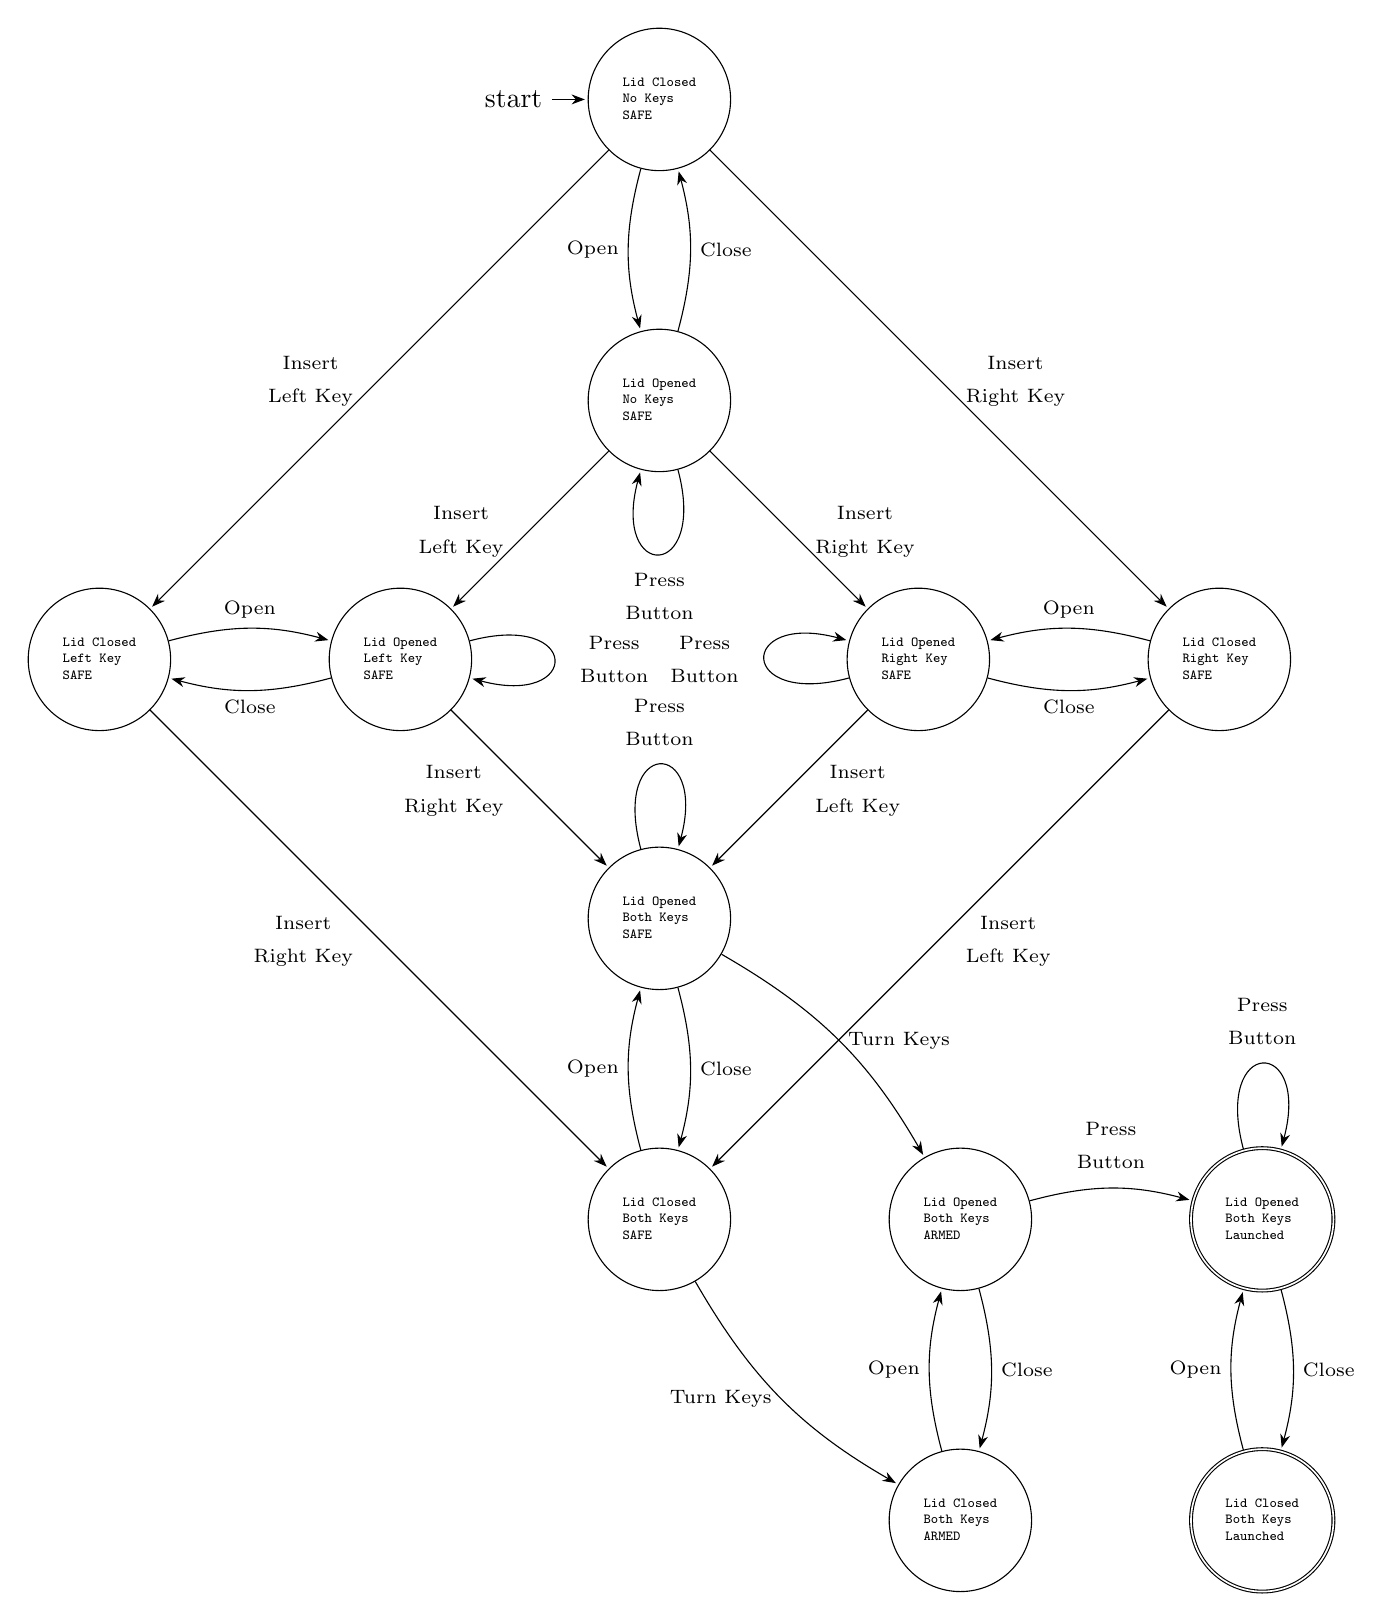
\begin{tikzpicture}[
    >=Stealth,
    shorten >=1pt,
    every state/.style={
        draw,
        minimum size=10mm,
        font=\tiny\ttfamily
    }
]
%\tikzstyle{every state}=[draw=black, scale=0.9, every node/.style={scale=0.9}]

% ---------------- SAFE REGION ----------------
\node[state, initial]   (CNS)                                       {\begin{tabular}{l} \tiny\ttfamily Lid Closed \\ \tiny\ttfamily No Keys   \\ \tiny\ttfamily SAFE     \end{tabular}};
\node[state]            (ONS) [below       =2.0cm           of CNS] {\begin{tabular}{l} \tiny\ttfamily Lid Opened \\ \tiny\ttfamily No Keys   \\ \tiny\ttfamily SAFE     \end{tabular}};
\node[state]            (OLS) [below left  =2.0cm and 2.0cm of ONS] {\begin{tabular}{l} \tiny\ttfamily Lid Opened \\ \tiny\ttfamily Left Key  \\ \tiny\ttfamily SAFE     \end{tabular}};
\node[state]            (ORS) [below right =2.0cm and 2.0cm of ONS] {\begin{tabular}{l} \tiny\ttfamily Lid Opened \\ \tiny\ttfamily Right Key \\ \tiny\ttfamily SAFE     \end{tabular}};
\node[state]            (OBS) [below right =2.0cm and 2.0cm of OLS] {\begin{tabular}{l} \tiny\ttfamily Lid Opened \\ \tiny\ttfamily Both Keys \\ \tiny\ttfamily SAFE     \end{tabular}};
\node[state]            (CLS) [      left  =2.0cm           of OLS] {\begin{tabular}{l} \tiny\ttfamily Lid Closed \\ \tiny\ttfamily Left Key  \\ \tiny\ttfamily SAFE     \end{tabular}};
\node[state]            (CRS) [      right =2.0cm           of ORS] {\begin{tabular}{l} \tiny\ttfamily Lid Closed \\ \tiny\ttfamily Right Key \\ \tiny\ttfamily SAFE     \end{tabular}};
\node[state]            (CBS) [below       =2.0cm           of OBS] {\begin{tabular}{l} \tiny\ttfamily Lid Closed \\ \tiny\ttfamily Both Keys \\ \tiny\ttfamily SAFE     \end{tabular}};
\node[state]            (OBA) [      right =2.0cm           of CBS] {\begin{tabular}{l} \tiny\ttfamily Lid Opened \\ \tiny\ttfamily Both Keys \\ \tiny\ttfamily ARMED    \end{tabular}};
\node[state]            (CBA) [below       =2.0cm           of OBA] {\begin{tabular}{l} \tiny\ttfamily Lid Closed \\ \tiny\ttfamily Both Keys \\ \tiny\ttfamily ARMED    \end{tabular}};
\node[state, accepting] (CBL) [      right =2.0cm           of CBA] {\begin{tabular}{l} \tiny\ttfamily Lid Closed \\ \tiny\ttfamily Both Keys \\ \tiny\ttfamily Launched \end{tabular}};
\node[state, accepting] (OBL) [      right =2.0cm           of OBA] {\begin{tabular}{l} \tiny\ttfamily Lid Opened \\ \tiny\ttfamily Both Keys \\ \tiny\ttfamily Launched \end{tabular}};

% Open Lid:
\draw[->] (CNS) to[bend right=15] node[left ] {\scriptsize Open}      (ONS);
\draw[->] (CLS) to[bend left =15] node[above] {\scriptsize Open}      (OLS);
\draw[->] (CRS) to[bend right=15] node[above] {\scriptsize Open}      (ORS);
\draw[->] (CBS) to[bend left =15] node[left ] {\scriptsize Open}      (OBS);
\draw[->] (CBA) to[bend left =15] node[left ] {\scriptsize Open}      (OBA);
\draw[->] (CBL) to[bend left =15] node[left ] {\scriptsize Open}      (OBL);

% Close Lid:
\draw[->] (ONS) to[bend right=15] node[right] {\scriptsize Close}     (CNS);
\draw[->] (OLS) to[bend left =15] node[below] {\scriptsize Close}     (CLS);
\draw[->] (ORS) to[bend right=15] node[below] {\scriptsize Close}     (CRS);
\draw[->] (OBS) to[bend left =15] node[right] {\scriptsize Close}     (CBS);
\draw[->] (OBA) to[bend left =15] node[right] {\scriptsize Close}     (CBA);
\draw[->] (OBL) to[bend left =15] node[right] {\scriptsize Close}     (CBL);

% SAFE: press (no effect, open only)
\draw[->] (ONS) edge[loop below]  node        {\begin{tabular}{c}\scriptsize Press \\ \scriptsize Button\end{tabular}    } ();
\draw[->] (OLS) edge[loop right]  node        {\begin{tabular}{c}\scriptsize Press \\ \scriptsize Button\end{tabular}    } ();
\draw[->] (ORS) edge[loop left ]  node        {\begin{tabular}{c}\scriptsize Press \\ \scriptsize Button\end{tabular}    } ();
\draw[->] (OBS) edge[loop above]  node        {\begin{tabular}{c}\scriptsize Press \\ \scriptsize Button\end{tabular}    } ();
\draw[->] (OBL) edge[loop above]  node        {\begin{tabular}{c}\scriptsize Press \\ \scriptsize Button\end{tabular}    } ();

% SAFE: Insert keys
\draw[->] (CNS) to[]              node[left ] {\begin{tabular}{c}\scriptsize Insert \\ \scriptsize Left  Key\end{tabular}} (CLS);
\draw[->] (CNS) to[]              node[right] {\begin{tabular}{c}\scriptsize Insert \\ \scriptsize Right Key\end{tabular}} (CRS);
\draw[->] (ONS) to[]              node[left ] {\begin{tabular}{c}\scriptsize Insert \\ \scriptsize Left  Key\end{tabular}} (OLS);
\draw[->] (ONS) to[]              node[right] {\begin{tabular}{c}\scriptsize Insert \\ \scriptsize Right Key\end{tabular}} (ORS);
\draw[->] (ORS) to[]              node[right] {\begin{tabular}{c}\scriptsize Insert \\ \scriptsize Left  Key\end{tabular}} (OBS);
\draw[->] (OLS) to[]              node[left ] {\begin{tabular}{c}\scriptsize Insert \\ \scriptsize Right Key\end{tabular}} (OBS);
\draw[->] (CRS) to[]              node[right] {\begin{tabular}{c}\scriptsize Insert \\ \scriptsize Left  Key\end{tabular}} (CBS);
\draw[->] (CLS) to[]              node[left ] {\begin{tabular}{c}\scriptsize Insert \\ \scriptsize Right Key\end{tabular}} (CBS);

% ARMED: Turn keys
\draw[->] (OBS) to[bend left =15] node[right] {\scriptsize Turn Keys} (OBA);
\draw[->] (CBS) to[bend right=15] node[left ] {\scriptsize Turn Keys} (CBA);

% Launch: Push button
\draw[->] (OBA) to[bend left =15] node[above] {\begin{tabular}{c} \scriptsize Press \\ \scriptsize Button\end{tabular}}     (OBL);

\end{tikzpicture}
\end{center}

\end{document}
